
\subsection{Kapitel 5}
\begin{figure}[ht]
    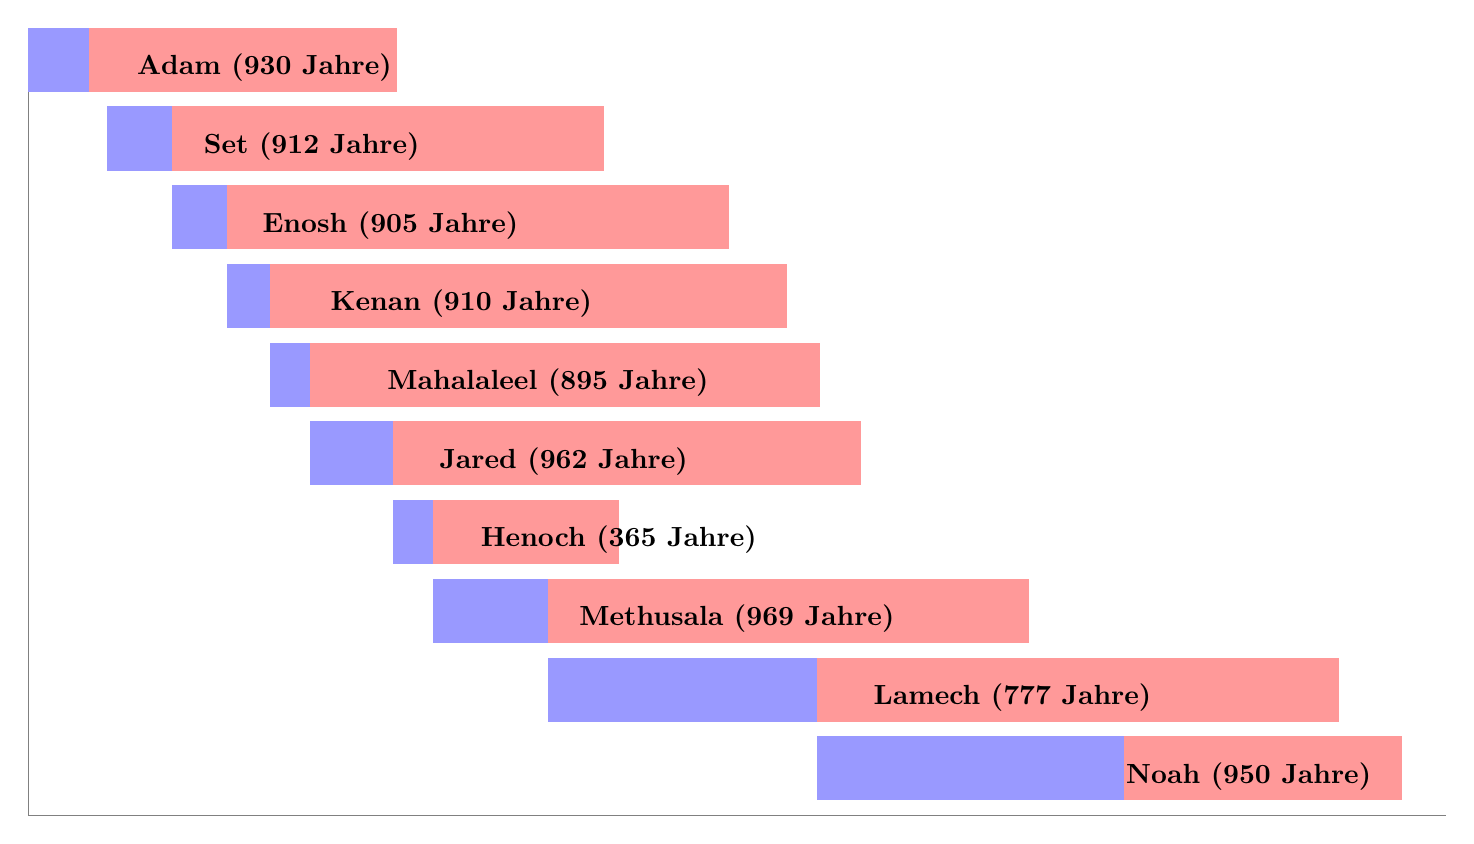
\begin{tikzpicture}
        \draw[gray] (0,0) -- (0mm, 100mm);
        %Adam 130-800 (10.1 - 62.4)
        \filldraw[blue!40] (0,100mm) rectangle(7.8mm,92mm);
        \filldraw[red!40] (7.8mm,100mm) rectangle(46.8mm,92mm) node at (30mm, 92mm) [right, above, black]{\textbf{Adam (930 Jahre)}};
        %Set 105-807 (8.19 - 62.9)
        \filldraw[blue!40] (10.1mm,90mm) rectangle(18.29mm,82mm);
        \filldraw[red!40] (18.29mm,90mm) rectangle(73.0mm,82mm) node at (36mm, 82mm) [right, above, black]{\textbf{Set (912 Jahre)}};
        %Enosch 90 - 815 (7.02 - 63.6)	
        \filldraw[blue!40] (18.29mm,80mm) rectangle (25.31mm,72mm);
        \filldraw[red!40] (25.31mm,80mm) rectangle(88.91mm,72mm) node at (46mm, 72mm) [right, above, black]{\textbf{Enosh (905 Jahre)}};
        %Kenan 70 - 840 (5.46 - 65.52)		
        \filldraw[blue!40] (25.31mm,70mm) rectangle(30.77mm,62mm);
        \filldraw[red!40] (30.77mm,70mm) rectangle(96.29mm,62mm) node at (55mm, 62mm) [right, above, black]{\textbf{Kenan (910 Jahre)}};
        %Mahalaleel 65 - 830 (5.07 - 64.7)
        \filldraw[blue!40] (30.77mm,60mm) rectangle(35.84mm,52mm);
        \filldraw[red!40] (35.84mm,60mm) rectangle(100.54mm,52mm) node at (66mm, 52mm) [right, above, black]{\textbf{Mahalaleel (895 Jahre)}};
        %Jared 162 - 800 (12.6 - 62.4)
        \filldraw[blue!40] (35.84mm,50mm) rectangle(46.44mm,42mm);
        \filldraw[red!40] (46.44mm,50mm) rectangle(105.68mm,42mm) node at (68mm, 42mm) [right, above, black]{\textbf{Jared (962 Jahre)}};
        %Henoch 65 - 300 (5.07 - 23.4)
        \filldraw[blue!40] (46.44mm,40mm) rectangle(51.51mm,32mm);
        \filldraw[red!40] (51.51mm,40mm) rectangle(74.91mm,32mm) node at (75mm, 32mm) [right, above, black]{\textbf{Henoch (365 Jahre)}};
        %Methusalah 187 - 782 (14.58 - 60.99)
        \filldraw[blue!40] (51.51mm,30mm) rectangle(66.09mm,22mm);
        \filldraw[red!40] (66.09mm,30mm) rectangle(127.08mm,22mm) node at (90mm, 22mm) [right, above, black]{\textbf{Methusala (969 Jahre)}};
        %Lamech 182 - 595 (14.19 - 46.41)
        \filldraw[blue!40] (66.09mm,20mm) rectangle(100.28mm,12mm);
        \filldraw[red!40] (100.28mm,20mm) rectangle(166.37mm,12mm) node at (125mm, 12mm) [right, above, black]{\textbf{Lamech (777 Jahre)}};
        % Noah 500 - 450 (39 - 35.1)
        \filldraw[blue!40] (100.28mm,10mm) rectangle(139.28mm,2mm);
        \filldraw[red!40] (139.28mm,10mm) rectangle(174.38mm,2mm) node at (155mm, 2mm) [right, above, black]{\textbf{Noah (950 Jahre)}};

        \draw[gray] (0,0) -- (180mm, 0mm);
    \end{tikzpicture}
    \caption{Lebensjahre bis Noah}
    \label{balken_alter}
\end{figure}
In diesem Kapitel wird das Geschlechtsregister Adams bis Noah aufgelistet. Die Menschen wurden zu der Zeit ziemlich alt. Durch dieses Alter gab es eine Spezielle konstellation.
Es ist interessant zu sehen (Abbildung: \ref{balken_alter}), wie Noah noch die Geburt von Lamech knapp miterleben konnte. Ich glaube zwar nicht, dass die sich nach so langer Zeit noch gekannt haben, aber es ist spannend. Am Ende das blauen Balken wurde dann der erste Sohn geboren, oder wenigsten die Person die die direkte Linie zu Jesus weiter führte.
Dieses Kapitel endet mit der Erwähnung von Noah und es werden seine Söhne Sem, Ham, Japhet aufgelistet.